\usepackage{xcolor}
\usepackage{afterpage}
\usepackage{pifont,mdframed}
\usepackage[bottom]{footmisc}
\usepackage[labelformat=empty]{caption}

\createsection{\Grader}{Test grader}

\renewcommand{\inputfile}{\texttt{stdin}}
\renewcommand{\outputfile}{\texttt{stdout}}
\makeatletter
\renewcommand{\this@inputfilename}{\texttt{stdin}}
\renewcommand{\this@outputfilename}{\texttt{stdout}}
\makeatother

\newenvironment{warning}
  {\par\begin{mdframed}[linewidth=2pt,linecolor=gray]%
    \begin{list}{}{\leftmargin=1cm
                   \labelwidth=\leftmargin}\item[\Large\ding{43}]}
  {\end{list}\end{mdframed}\par}
\newenvironment{danger}
{\par\begin{mdframed}[linewidth=2pt,linecolor=red!60!yellow,backgroundcolor=red!20!white]%
		\begin{list}{}{\leftmargin=1cm
				\labelwidth=\leftmargin}\item[\Large\ding{45}]}
		{\end{list}\end{mdframed}\par}

% % % % % % % % % % % % % % % % % % % % % % % % % % % % % % % % % % % % % % % % % % %
% % % % % % % % % % % % % % % % % % % % % % % % % % % % % % % % % % % % % % % % % % %

The Italian Olympiad in Informatics committee thinks that this year's tasks might
be a tad too easy. For this reason, the contest venue in Campobasso and the
hotel were placed on a $N \times N$ grid, where each cell is highly flammable.
The hotel is placed at the coordinates $(0,0)$, while the contest venue is
placed at the coordinates $(N-1, N-1)$. Thus, besides solving the problems, our
contestants this year will also have to avoid the fires they will encounter on the
way from the hotel to the contest venue.

The committee managed to get the permission by the city council to start
\emph{at the same time} $M$ fires, numbered from $0$ to $M-1$. The $i$-th fire
starts at the coordinates $(X[i], Y[i])$. For every minute passed, every cell on
fire will ignite a new fire inside its four adjacent cells (north, south, east,
west), if those weren't on fire already. The fires will spread on the grid until
it is completely on fire, but they are controlled so that they won't escape the
grid (for public safety reasons).

\begin{figure}[h]
    \begin{center}
  \begin{minipage}{0.45\linewidth}
    \includegraphics[width=\linewidth]{asy_incendio/es1.pdf}
    \caption*{Situation at the beginning}
  \end{minipage}
  \hspace{0.05\linewidth}
  \begin{minipage}{0.45\linewidth}
    \includegraphics[width=\linewidth]{asy_incendio/es2.pdf}
    \caption*{Situation after a minute}
  \end{minipage}
  \end{center}
\end{figure}

For the contestants, clearly, it is better to leave the hotel as soon as possible
to have more chance to get to the content unharmed. Chupito, instead, like most
cats, is pathologically lazy and doesn't want to get up early unless strictly
necessary.

At any moment Chupito can move to one of the four cells adjacent to its current
location, but he cannot exit the grid, and cannot go across any cell which is on
fire. In order to sleep as much as possible, Chupito wants to leave the hotel at
the latest possible time.

Help Chupito! Compute \textbf{after how many minutes at most} after the fires
are started there is still some route to reach the contest venue.

% % % % % % % % % % % % % % % % % % % % % % % % % % % % % % % % % % % % % % % % % % %
% % % % % % % % % % % % % % % % % % % % % % % % % % % % % % % % % % % % % % % % % % %

\pagebreak
\Implementation

You have to submit one file, with extension \texttt{.c} or \texttt{.cpp}.

\begin{warning}
	You will find among the attachments the templates \texttt{incendio.c} and \texttt{incendio.cpp} with an implementation example.
\end{warning}

You have to implement the following function:

\begin{center}\begin{tabularx}{\textwidth}{|c|X|}
\hline
C/C++  & \verb|int alzati(int N, int M, int X[], int Y[]);|\\
\hline
\end{tabularx}\end{center}

\begin{itemize}[nolistsep]
  \item The integer $N$ is the dimension of the city grid.
  \item The integer $M$ is the number of fires started initially.
  \item The arrays \texttt{X} e \texttt{Y} (indexed from $0$ to $M-1$) contain
  	    the initial coordinates of the $M$ fires. The $i$-th fire starts at the
  	    coordinates $(X[i], Y[i])$.
  \item The function must return an integer representing the maximum number of
  		minutes after which it is still possible to reach the contest venue
  		safely.
\end{itemize}

\medskip

The grader will call the function \texttt{alzati} and will print its return
value to the output.

% % % % % % % % % % % % % % % % % % % % % % % % % % % % % % % % % % % % % % % % % % %
% % % % % % % % % % % % % % % % % % % % % % % % % % % % % % % % % % % % % % % % % % %


\Grader

In the task folder there is a simplified version of the grader used during
evaluation. You can use this sample grader to test your solutions locally. This
grader reads the input from \inputfile{}, calls the functions you implemented,
and writes the output on \outputfile{}.

The input file is formed by $M+1$ lines, each with the following:
\begin{itemize}[nolistsep,itemsep=2mm]
\item Line $1$: the integers $N$ and $M$ separated by a space.
\item Each of the following $M$ lines: the values \texttt{X[$i$]} and \texttt{Y[$i$]}, separated by a space, for $i = 0\ldots M-1$.
\end{itemize}

The output file is formed by a single line, with:
\begin{itemize}[nolistsep,itemsep=2mm]
\item Line $1$: the value returned by function \texttt{alzati}.
\end{itemize}

% % % % % % % % % % % % % % % % % % % % % % % % % % % % % % % % % % % % % % % % % % %
% % % % % % % % % % % % % % % % % % % % % % % % % % % % % % % % % % % % % % % % % % %


\Constraints

\begin{itemize}[nolistsep, itemsep=2mm]
	\item $2 \le N \le 1\,000\,000\,000$.
	\item $1 \le M \le 12\,000$.
	\item $0 \le X[i], Y[i] \le N-1$ for each $i = 0, \ldots, M-1$.
	\item All the fires start from distinct coordinates.
	\item Initially, it is possible to reach the contest venue.
	\item Initially, there are no fires at the coordinates $(0,0)$ and $(N-1, N-1)$.
\end{itemize}

% % % % % % % % % % % % % % % % % % % % % % % % % % % % % % % % % % % % % % % % % % %
% % % % % % % % % % % % % % % % % % % % % % % % % % % % % % % % % % % % % % % % % % %

\Scoring

Your program will be tested on several test cases grouped in subtask. To
achieve the score of a subtask, you need to correctly solve all of its test cases.


\begin{itemize}[nolistsep,itemsep=2mm]
  \item \textbf{\makebox[2cm][l]{Subtask 1} [\phantom{1}0 points]}: Sample cases.
  \item \textbf{\makebox[2cm][l]{Subtask 2} [\phantom{1}7 points]}: $M=1$.
  \item \textbf{\makebox[2cm][l]{Subtask 3} [10 points]}: $X[i] = X[j]$ for every $0 \leq i, j < M$.
  \item \textbf{\makebox[2cm][l]{Subtask 4} [20 points]}: $N \leq 500$.
  \item \textbf{\makebox[2cm][l]{Subtask 5} [22 points]}: $N \leq 1000$.
  \item \textbf{\makebox[2cm][l]{Subtask 6} [24 points]}: $M \leq 2000$ and $X[i] + Y[i]$ is even, for every $0 \leq i < M$.
  \item \textbf{\makebox[2cm][l]{Subtask 7} [\phantom{1}9 points]}: $M \leq 10\,000$.
  \item \textbf{\makebox[2cm][l]{Subtask 8} [\phantom{1}8 points]}: No additional limitations.
\end{itemize}

% % % % % % % % % % % % % % % % % % % % % % % % % % % % % % % % % % % % % % % % % % %
% % % % % % % % % % % % % % % % % % % % % % % % % % % % % % % % % % % % % % % % % % %

\Examples

\begin{example}
\exmpfile{incendio.input0.txt}{incendio.output0.txt}%
\exmpfile{incendio.input1.txt}{incendio.output1.txt}%
\end{example}

% % % % % % % % % % % % % % % % % % % % % % % % % % % % % % % % % % % % % % % % % % %
% % % % % % % % % % % % % % % % % % % % % % % % % % % % % % % % % % % % % % % % % % %


\Explanation

In the \textbf{first sample case} we have an $8 \times 8$ grid initially
containing $3$ fires. The grid evolves as follows.

\begin{center}
	\begin{minipage}{0.31\linewidth}
		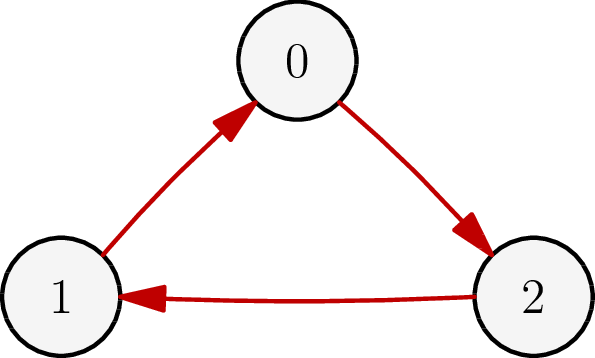
\includegraphics[width=\linewidth]{asy_incendio/fig1.pdf}
		\caption*{Situation at time $t=0$}
	\end{minipage}
	\hspace{0.02\linewidth}
	\begin{minipage}{0.31\linewidth}
		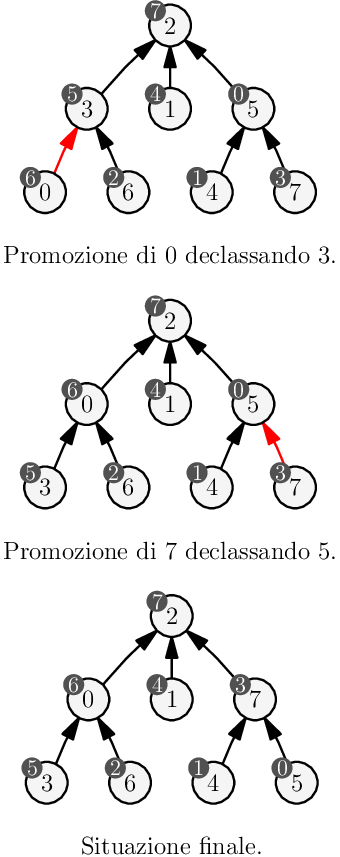
\includegraphics[width=\linewidth]{asy_incendio/fig2.pdf}
		\caption*{Situation at time $t=1$}
	\end{minipage}
	\hspace{0.02\linewidth}
	\begin{minipage}{0.31\linewidth}
		\includegraphics[width=\linewidth]{asy_incendio/fig3.pdf}
		\caption*{Situation at time $t=2$}
	\end{minipage}
\end{center}

Starting with time $t = 4$ it will not be possible to reach the contest venue
safely, so the time $t = 3$ is the last minute in which Chupito can get up.

\begin{center}
	\begin{minipage}{0.31\linewidth}
		\includegraphics[width=\linewidth]{asy_incendio/fig4.pdf}
		\caption*{Situation at time $t=3$}
	\end{minipage}
	\hspace{0.03\linewidth}
	\begin{minipage}{0.31\linewidth}
		\includegraphics[width=\linewidth]{asy_incendio/fig5.pdf}
		\caption*{Situation at time $t=4$}
	\end{minipage}
\end{center}

In the \textbf{second sample case}, after $t = 1$ it is already not possible to
reach the contest venue:

\begin{center}
	\begin{minipage}{0.3\linewidth}
		\includegraphics[width=\linewidth]{asy_incendio/fig6.pdf}
		\caption*{Situation at time $t=0$}
	\end{minipage}
	\hspace{0.03\linewidth}
	\begin{minipage}{0.3\linewidth}
		\includegraphics[width=\linewidth]{asy_incendio/fig7.pdf}
		\caption*{Situation at time $t=1$}
	\end{minipage}
	\hspace{0.03\linewidth}
	\begin{minipage}{0.3\linewidth}
		\includegraphics[width=\linewidth]{asy_incendio/fig8.pdf}
		\caption*{Situation at time $t=2$}
	\end{minipage}
\end{center}
